\clearpage
\section{Event display}
In this part, we focused into learning how to distinguish different channel by event display and four different variables. All channels have 20 events. 



\subsection{Identification of the particle at the OPAL detector}
To identify the particles, firstly, we divide all particle in charged and uncharged on the basis of visible trajectory.

The charged hadrons and electrons are separated on the basis of their form and beginning of the shower. The electromagnetic showers caused by an electron have small lateral spread and completely situated with in the electromagnetic calorimeter (ECAL); however, hadronic showers are wider and extended up to the hadronic calorimeter(HCAL). And, muons do not produce any shower.

 The neutral particles are identify with the help of different parameters of showers (length, width). The neutral particle decay in to charged particles and follow V tracks. Figure \ref{fig:signature} represent the signature of the particles. \\
 

The different decay channels are identified as:
\begin{enumerate}
\item $ \text{z}^0\rightarrow e^+e^- $\\
They create electromagnetic showers through Bremsstrahlung and deposit their energy in the electromagnetic calorimeter. 

\item $ \text{z}^0\rightarrow \mu^+\mu^- $\\ 
Muons are heaver than electrons, they don't show showers either Ecal nor Hcal. They penetrate the Hcal and trigger signal in the muon chambers.

\item $ \text{z}^0\rightarrow \tau^+\tau-$\\
Tau particles have short life time, so they decay quickly. They can be identified by their decay product. Since they are heavier than electrons and muon and their sum of momentum is less than that electrons and muons for the same energy.

\item $ \text{z}^0\rightarrow q\bar{q}$\\
Since quarks cannot exist freely and they form jet of hadrons via strong interaction. Hadronic events have high charge tracks, so they are easy identified.
\end{enumerate}

In this part we can measured the following variables for each event:
\begin{itemize}
	\item Ctrk(N): Number of charged tracks
	\item Ctrk(SumP): Momentum of all charged tracks
	\item Ecal(SumE): Total energy deposited in the electromagnetic calorimeter
	\item Hcal(SumE): Total energy deposited in the hadronic calorimeter
\end{itemize}
The measured values for each events of channels: $ \text{z}^0\rightarrow e^+e^- $, $ \text{z}^0\rightarrow \mu^+\mu^- $, $ \text{z}^0\rightarrow \tau^+\tau-$,  and $ \text{z}^0\rightarrow  $  of $ z^0 $ boson are, respectively, listed in Tables \ref{tab:ee}, \ref{tab:mm}, \ref{tab:tt}, and \ref{tab:qq} in the appendix. Figure \ref{fig:eventsDisplay} shows the GROUPE output of different decay channels.



\begin{figure}[H]   
	\begin{minipage}[t]{0.5\textwidth}
		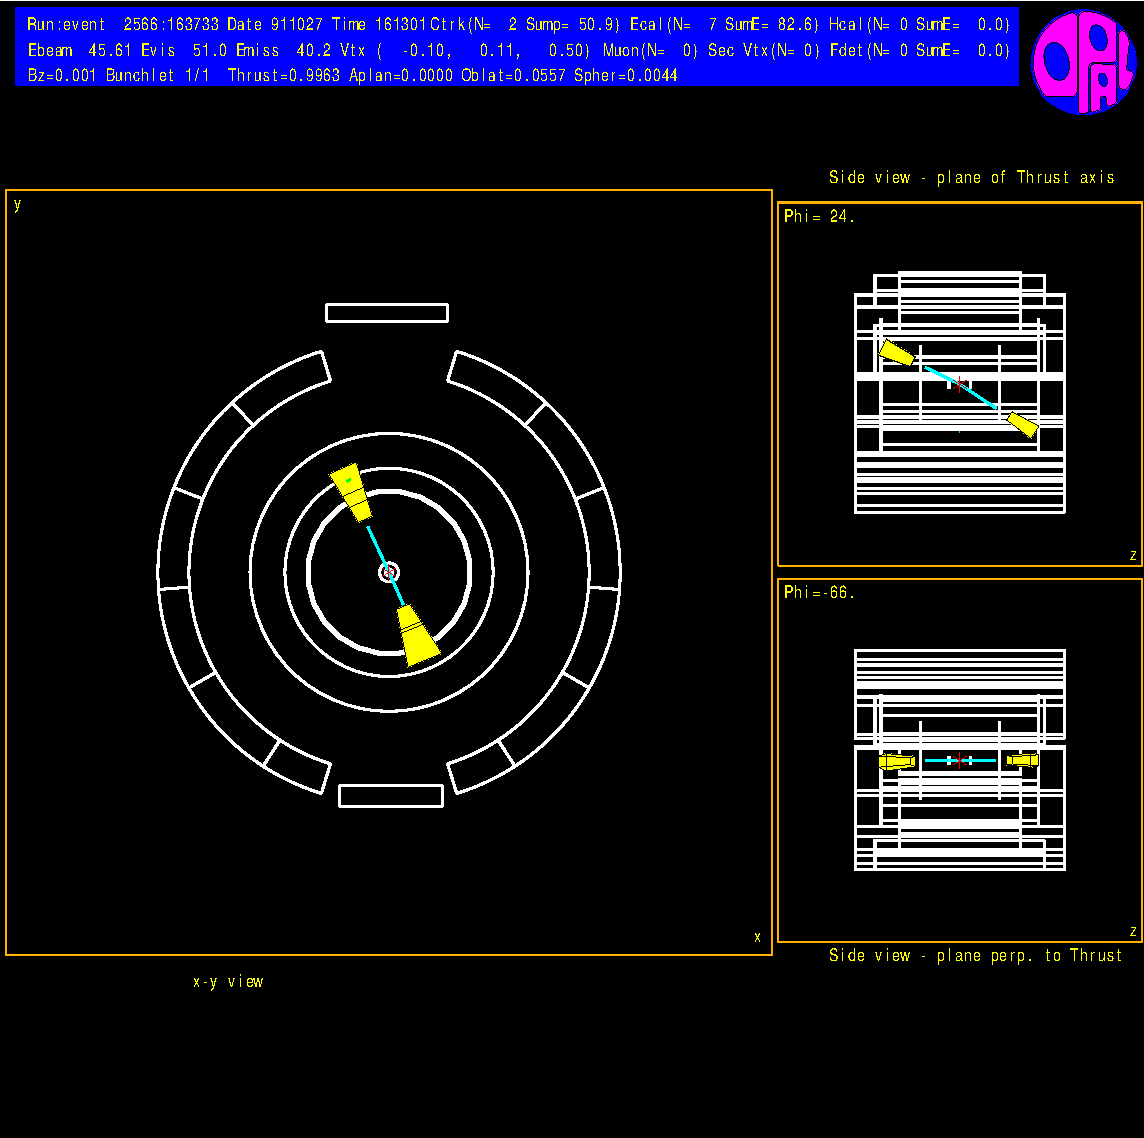
\includegraphics[width=\linewidth]{ee_1.pdf}
		\begin{center}
			{(a) $  \text{z}^0\rightarrow e^+e^- $}
		\end{center}
	\end{minipage} \quad
	\begin{minipage}[t]{0.5\textwidth}
		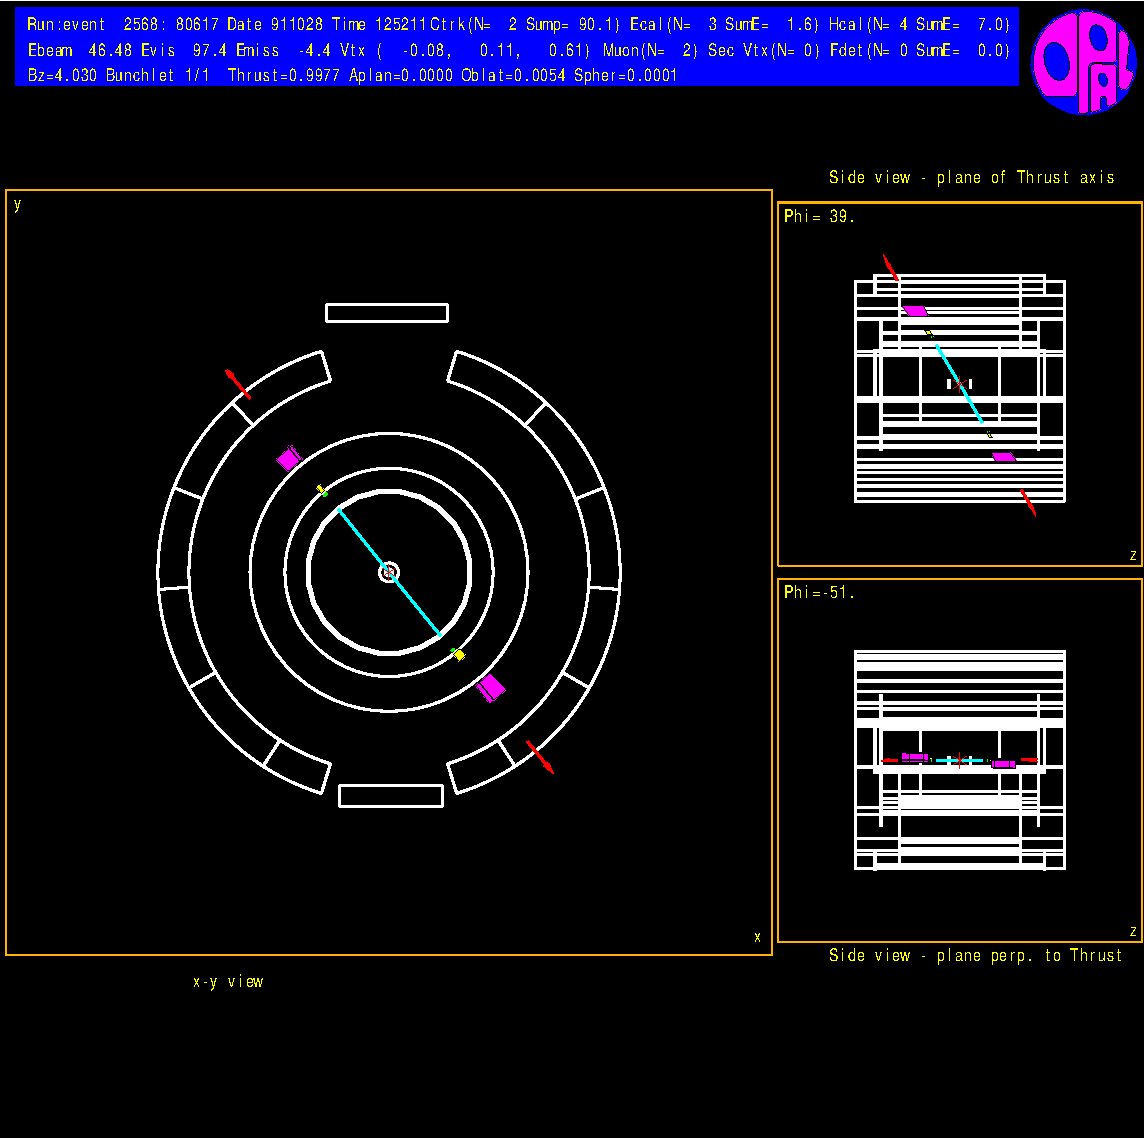
\includegraphics[width=\linewidth]{mm_1.pdf}
		\begin{center}
			{(b) $ \text{z}^0\rightarrow \mu^+\mu^- $}
		\end{center}
	\end{minipage}\\\\
	
	
	\begin{minipage}[t]{0.5\textwidth}
		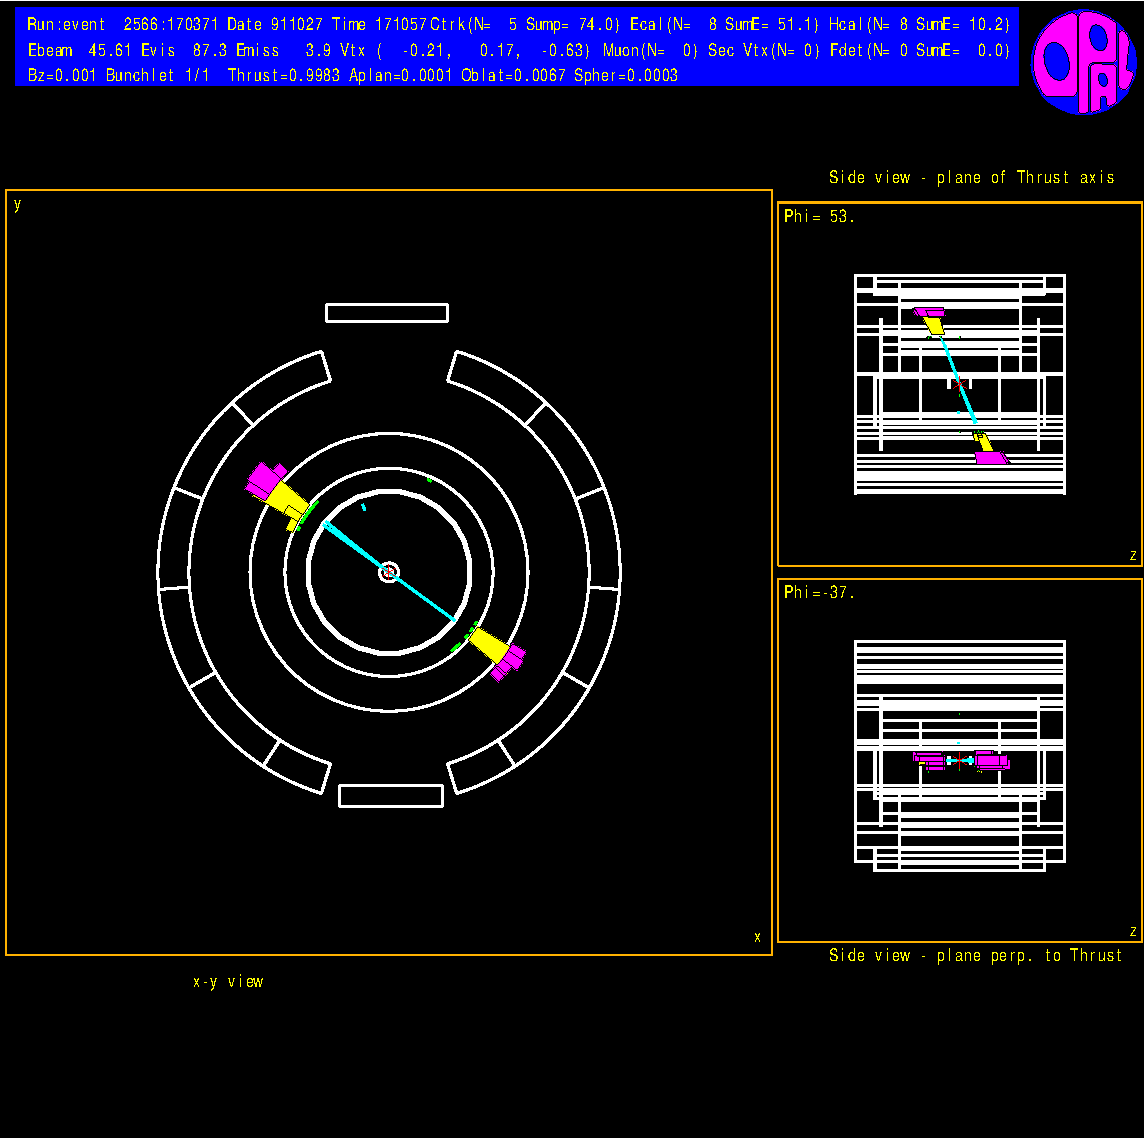
\includegraphics[width=\linewidth]{tt_1.pdf}
		\begin{center}
			{(c) $ \text{z}^0\rightarrow \tau^+\tau^- $}
		\end{center}
	\end{minipage} \quad
\begin{minipage}[t]{0.5\textwidth}
		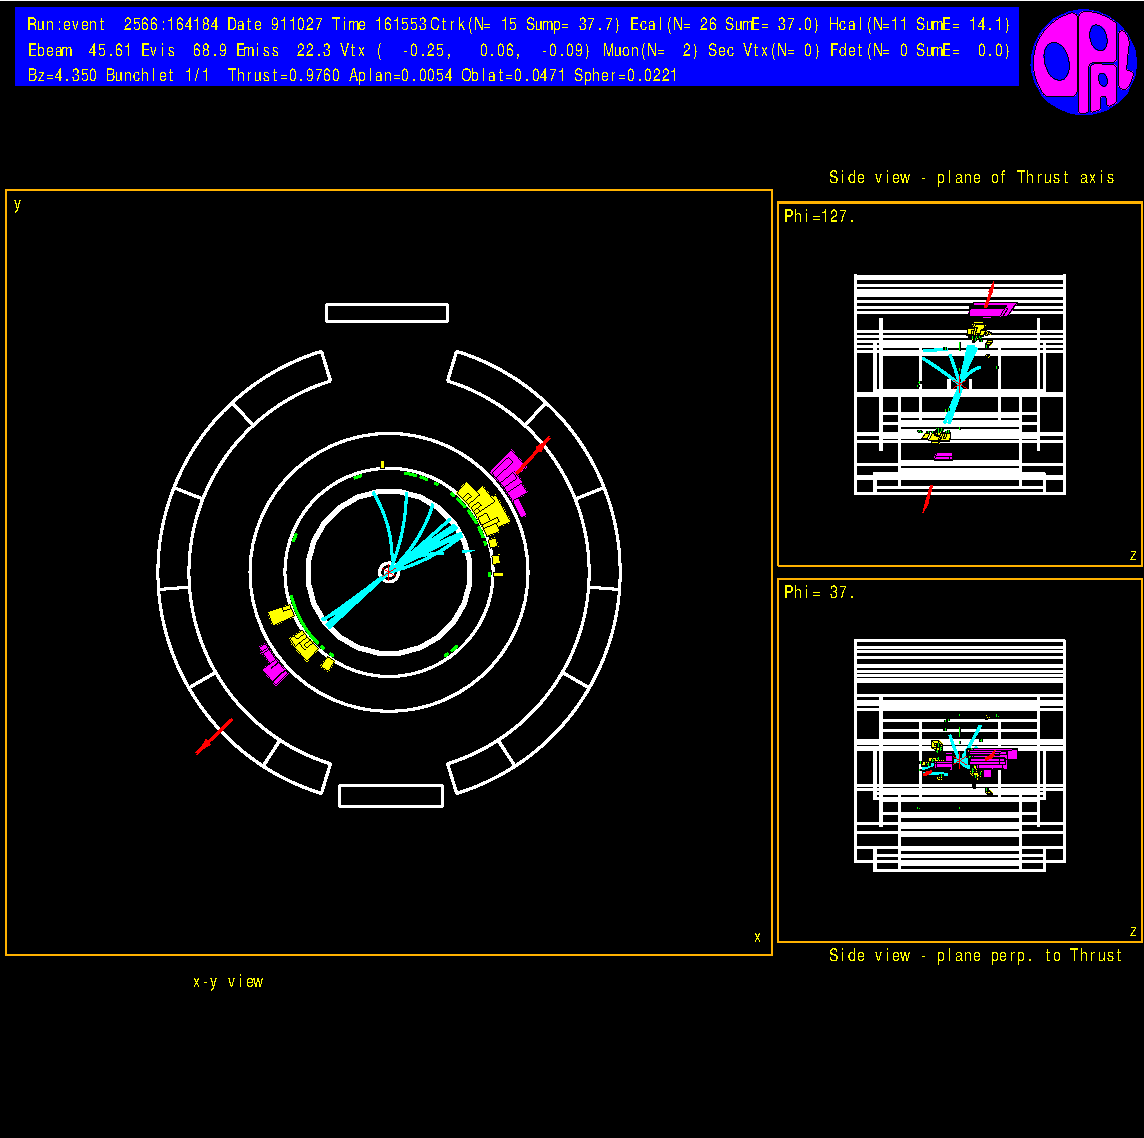
\includegraphics[width=\linewidth]{qq_1.pdf}
		\begin{center}
			{(d) $ \text{z}^0\rightarrow q \bar{q}$}
		\end{center}
	\end{minipage}
\caption{ GROPE output of four different decay modes of $ Z^0 $ boson.}
\label{fig:eventsDisplay}	
\end{figure}

\subsection{Determination of appropriate cuts for events classification}
We plotted the histograms for different parameters of different channels and used to choose the appropriate cuts. Figure \ref{Fig:histograms} shows Histograms of different variables measured in $  \text{z}^0\rightarrow e^+e^- $ channel. From histograms we set the cuts to optical separation of the $ \text{Z}^0 $ decays of different channels. For this we have chosen acceptance of cuts (AC) as
\begin{equation}
AC= \frac{\text{The events of a certain class fullfilling the cut criterion}}{\text{Total number of events of the same class}}
\end{equation}
Hence our taken cuts are listed in table \ref{Tab:cuts}

  
\begin{figure}[H]   
	\begin{minipage}[t]{0.5\textwidth}
		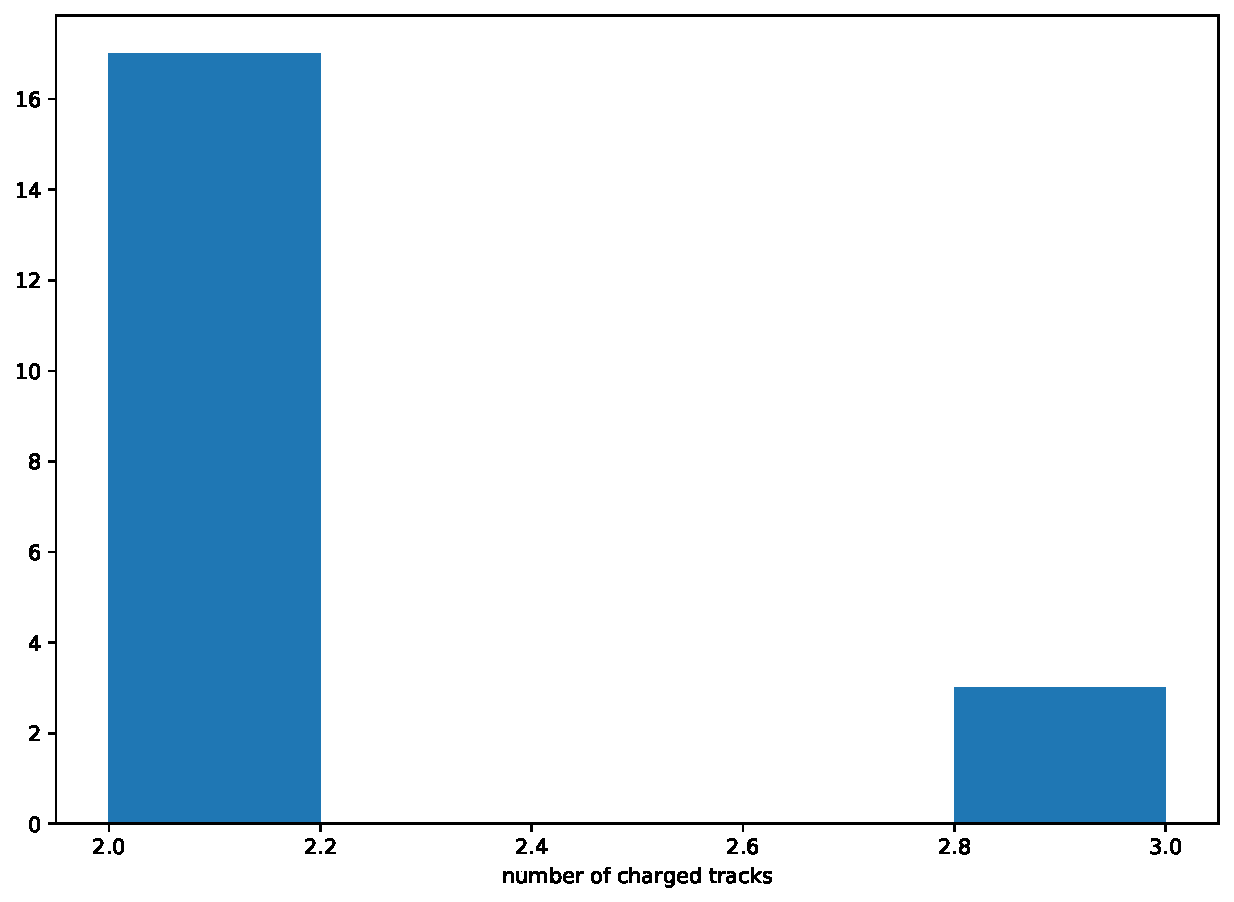
\includegraphics[width=\linewidth]{ee_Ctrk_N.pdf}
		\begin{center}
			{(a) Histogram showing the number of charge tracks}
		\end{center}
	\end{minipage} \quad
	\begin{minipage}[t]{0.5\textwidth}
		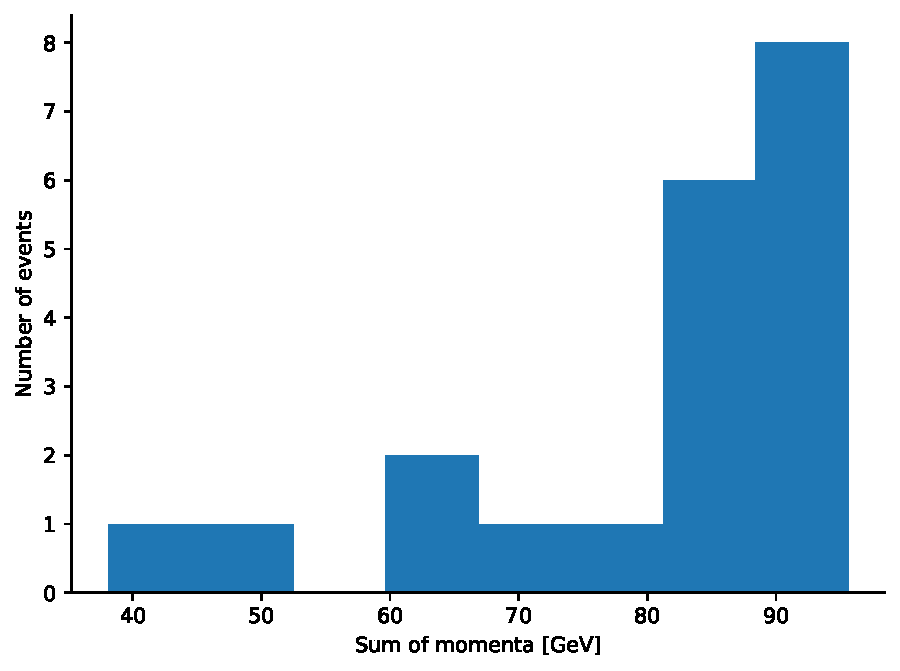
\includegraphics[width=\linewidth]{ee_Ctrl_Sump.pdf}
		\begin{center}
			{(b) Histogram showing the total scalar sum of track momenta}
		\end{center}
	\end{minipage}\\\\
	
	
	\begin{minipage}[t]{0.5\textwidth}
		\includegraphics[width=\linewidth]{ee_Ecal.pdf}
		\begin{center}
			{(c) Histogram showing the energy deposited in the Electromagnetic Calorimeter}
		\end{center}
	\end{minipage} \quad
	\begin{minipage}[t]{0.5\textwidth}
		\includegraphics[width=\linewidth]{ee_Hcal.pdf}
		\begin{center}
			{(d) Histogram showing the energy deposited in the Hadronic Calorimeter}
		\end{center}
	\end{minipage}
	\caption{Histograms of different variables measured in $  \text{Z}^0\rightarrow e^+e^- $ channel. Here y-axis represent the number of events in all histograms.}
\label{Fig:histograms}	
\end{figure}

\begin{table}[H]
	\centering
	\begin{tabular}{ccc ccc}
		\toprule
		Particle & Ctrk(N) & Ctrk(Sump) & Ecal(SumE) & Hcal(SumE) \\
		\midrule
		Electrons & $ \le $ 3 &   &    \textgreater 50  & \textless 1	\\
		Muons &  $ \le $ 3 &  $ \ge $50  &    \textless 10  & \textless 30	\\
		Tauon &  $ \le $ 7 & \textless 75  & \textless 60    & \textless 30	\\
		Hadrons &  $ \ge $7 &   &  \textgreater 30    &	\\
		
		\bottomrule
	\end{tabular}
	\caption{Measured Cuts for different variables of different channels.}
	\label{Tab:cuts}
\end{table}
\subsection{Event classification for test sample}


	
To classify events from the sample test1 we used the cuts from table \ref{Tab:cuts}. To do so, firstly, we checked the  CtrkN to pick out hadrons particle from others, also we verified  Ecal number. Secondly, we check the values of Ecal and Hcal to verified electrons. Finally, we checked the value of CtrkSump as well as  Ecal and Hcal to conform the muons or tauons. The measured valued for each variables and the decay channel clasification result are given table \ref{tab:test1}.

\begin{table*}[htbp]
	\centering
	
	\begin{tabular}{ccc ccc}
		\toprule
		Event & Ctrk(N) & Ctrk(Sump) & Ecal(SumE) & Hcal(SumE) & Comment \\
		\midrule

1& 19& 39.5&44.3&15.6 & $ \text{z}^0\rightarrow q\bar{q}$\\
2& 36& 42.8&57.1&12.5& $ \text{z}^0\rightarrow q \bar{q}$\\
3& 2& 95.7& 93.4&0.0& $ \text{z}^0\rightarrow e^+e^- $\\
4& 2& 90.8&1.4&4.1& $ \text{z}^0\rightarrow \mu^+\mu^- $\\
5& 4& 36.5&35.8&10.8& $ \text{z}^0\rightarrow \tau^+\tau-$\\
6& 2& 97.0&2.2&8.9& $ \text{z}^0\rightarrow \mu^+\mu^- $\\
7& 68& 42.9&48.5&6.2& $ \text{z}^0\rightarrow q\bar{q}$\\
8& 5& 35.0&40.8&3,3& $ \text{z}^0\rightarrow \tau^+\tau-$\\
9& 21& 75.8&45.8&21.0&$ \text{z}^0\rightarrow q \bar{q}$\\
10& 2& 95.2&1.3&7.9& $ \text{z}^0\rightarrow e^+e^- $\\
11& 2& 22.7&34.4&0.0& $ \text{z}^0\rightarrow \tau^+\tau-$\\
12& 4& 44.3&37.8&2.6& $ \text{z}^0\rightarrow \tau^+\tau-$\\
13& 21& 53.1&36.2&22.9& $ \text{z}^0\rightarrow q\bar{q}$\\
14& 2& 89.5&92.0&0.0& $ \text{z}^0\rightarrow e^+e^- $\\
15& 2& 89.1&89.7&0.0& $ \text{z}^0\rightarrow e^+e^- $\\
16& 2& 4.1&4.4&0.0& $ \text{z}^0\rightarrow \tau^+\tau-$\\
17& 2& 87.8&1.4&4.3& $ \text{z}^0\rightarrow \mu^+\mu^- $\\
18& 2& 75.3&90.0&0.0& $ \text{z}^0\rightarrow e^+e^- $\\
19& 2& 93.7&1.6&6.8& $ \text{z}^0\rightarrow \mu^+\mu^- $\\
20& 2& 67.1&93.6&0.0& $ \text{z}^0\rightarrow e^+e^- $\\
\bottomrule
\end{tabular}
\caption{Measured parameter for $ \text{z}^0\rightarrow $ hadrons channel}
\label{tab:test1}
\end{table*}

